\documentclass[a4paper]{article}
\usepackage{amsmath, amsfonts}
\usepackage{tikz}
\usetikzlibrary{arrows, shapes}
\usetikzlibrary{decorations.pathmorphing}
\usetikzlibrary{calc,arrows.meta,positioning}

\begin{document}

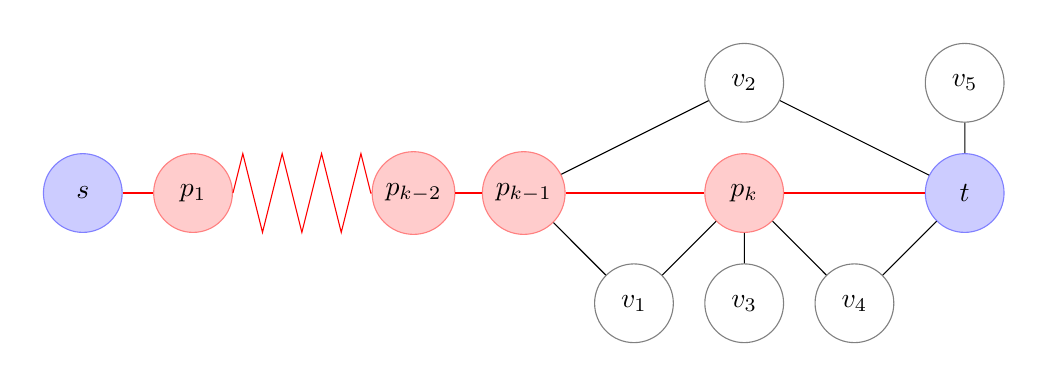
\begin{tikzpicture}[scale=1.4]
    \clip (-0.5,-1.5) rectangle (8.5,1.5);

    \begin{scope}[circle,minimum size=10mm]
        \node at (0, 0) [draw=blue!50,fill=blue!20] (s) {$s$};
        \node at (1, 0) [draw=red!50,fill=red!20] (1) {$p_1$};
        \node at (3, 0) [draw=red!50,fill=red!20] (k-2) {$p_{k - 2}$};
        \node at (4, 0) [draw=red!50,fill=red!20] (k-1) {$p_{k - 1}$};
        \node at (6, 0) [draw=red!50,fill=red!20] (k) {$p_{k}$};
        \node at (5, -1) [draw=black!50] (v1) {$v_1$};
        \node at (6, 1) [draw=black!50] (v2) {$v_2$};
        \node at (6, -1) [draw=black!50] (v3) {$v_3$};
        \node at (7, -1) [draw=black!50] (v4) {$v_4$};
        \node at (8, 1) [draw=black!50] (v5) {$v_5$};
        \node at (8, 0) [draw=blue!50,fill=blue!20] (t) {$t$};
    \end{scope}

    \path [every node/.style={font=\sffamily\small, sloped}]
    (s) edge [red] node [above] {} (1)
    (k-1) edge [red] node [above] {} (k)
    (k-2) edge [red] node [above] {} (k-1)
    (k-1) edge node [above] {} (v1)
    (k-1) edge node [above] {} (v2)
    (v2) edge node [above] {} (t)
    (v1) edge node [above] {} (k)
    (k) edge [red] node [above] {} (t)
    (k) edge node [above] {} (v3)
    (k) edge node [above] {} (v4)
    (v4) edge node [above] {} (t)
    (v5) edge node [above] {} (t);

    \draw [decorate, decoration={zigzag, segment length=5mm, amplitude=5mm}, red] (1) -- (k-2);

\end{tikzpicture}

\end{document}